\documentclass[tikz,border=2pt]{standalone}
\usepackage{amsmath}
\usepackage{pgfplots}
\pgfplotsset{compat=1.18}
\usetikzlibrary{arrows.meta}
\begin{document}
% Example 6.3: bases {5,6} -> {1,6} -> {1,2} -> {3,2} -> {3,4} -> {5,4} -> {5,6}; every basic solution is x=0
% with Z=0 and step length 0; steps 2, 4, 6 break a tie in the ratio test towards the lower row.
% The LP is unbounded along t(0,7,1,0) with Z=1.5t, a direction the cycle never takes.
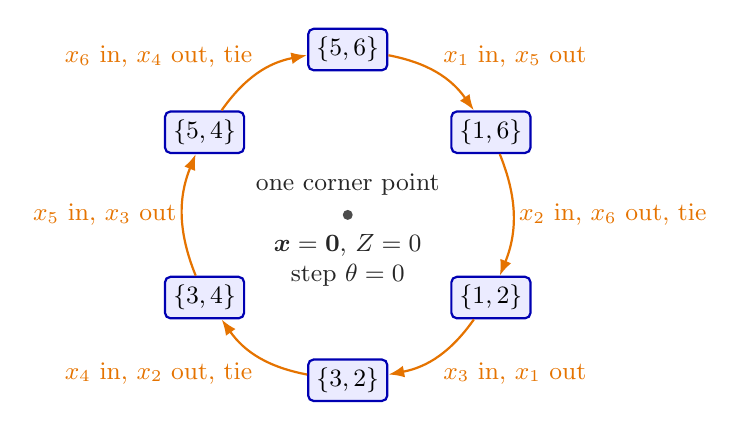
\begin{tikzpicture}[font=\small, >={Latex[length=2mm]},
    basis/.style={draw=blue!70!black, thick, fill=blue!8, rounded corners=2pt, inner sep=3pt}]
  \def\r{2.1}
  \foreach \k/\b in {0/{\{5,6\}},1/{\{1,6\}},2/{\{1,2\}},3/{\{3,2\}},4/{\{3,4\}},5/{\{5,4\}}}
    \node[basis] (b\k) at ({90-60*\k}:\r) {$\b$};
  % exchanges: entering in, leaving out
  \foreach \k/\n/\lab/\anc in {0/1/{$x_1$ in, $x_5$ out}/south west, 1/2/{$x_2$ in, $x_6$ out, tie}/west, 2/3/{$x_3$ in, $x_1$ out}/north west,
                               3/4/{$x_4$ in, $x_2$ out, tie}/north east, 4/5/{$x_5$ in, $x_3$ out}/east, 5/0/{$x_6$ in, $x_4$ out, tie}/south east} {
    \draw[->, thick, orange!90!black] (b\k) to[bend left=22] coordinate[pos=0.5] (m\k) (b\n);
    \node[orange!90!black, anchor=\anc, inner sep=2pt] at (m\k) {\lab};
  }
  % the corner point all bases share
  \fill[gray!60!black] (0,0) circle (1.8pt);
  \node[gray!30!black, anchor=north, align=center] at (0,-0.12) {$\boldsymbol{x}=\boldsymbol{0}$, $Z=0$\\ step $\theta=0$};
  \node[gray!30!black, anchor=south] at (0,0.12) {one corner point};
\end{tikzpicture}
\end{document}
